Now that the requirements necessary to build the system have been formulated, potential solutions to fulfil the list of requirements from Chapter \ref{ch:chapter3} for each aspect of the system can now be analysed before choosing a final solution. Throughout this chapter, the requirements established from the previous chapter referred as ``F'' stand for functional requirements, while requirements referred as ``NF'' stand for non-functional requirements. The first section of this chapter will focus on different solutions for the system's pipeline, starting with the offline feature extraction phase, followed by the online retrieval phase, and ending with the database pre-processing phase. The second section will focus on general design decisions such as the programming language, the query video pre-processing operations, the type of interface, the type of file to store the features in and the type of videos to use. These two sections are used to conclude with an outline of the final chosen solutions for each aspect of the system, which are used to bring the system to life.

\section{Pipeline Design Analysis}

To chose a global design solution for the system, it is easier to break down the system's pipeline into different phases and review the numerous potential designs for each of these phases. The system pipeline can be split into three different phases, as shown in the concise diagram in Figure \ref{fig:basic-cbvr-diagram}:

\begin{itemize}
    \item \textbf{Offline Feature Extraction Phase}. This phase corresponds to the ``training'' phase of the system, where features are extracted from each video in the database and then stored in data files for the retrieval phase.
    \item \textbf{Online Retrieval Phase}. This phase is affiliated to the ``training'' phase of the system, where a single video query is matched to one of the database videos by extracting the same features from the previous phase and comparing them to the stored features.
    \item \textbf{Database Pre-processing Phase}. This is an optional phase where the database videos are processed before the offline feature extraction phase to improve the accuracy and speed of the database videos feature extraction.
\end{itemize}

\begin{figure}[h]
\centerline{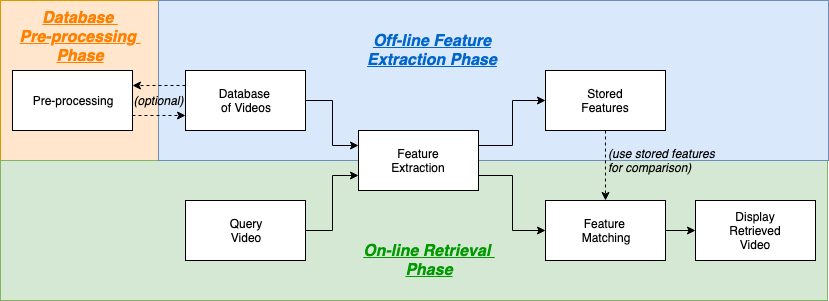
\includegraphics[width=\textwidth]{figures/design/basic_cbvr_phases.png}}
\caption{\label{fig:basic-cbvr-diagram}Basic CBVR system diagram.}
\end{figure}

\begin{comment}
Explore possible options for different sections of the system, such as:
    \begin{itemize}
        \item types of features to extract (why static colour features and not object/motion features) - histograms are very popular with videos, calculations are easier, implementation is easier, results are as efficient
        \item types of learning models (histogram matching, BoW-approach VS Neural Network)
    \end{itemize}
\end{comment}

\subsection{Offline Feature Extraction Phase}
\label{sec:design-offline-feature-extraction}

The first distinction between the possible types of features that could be extracted from the videos is static and dynamic features. Because static features extraction are a much less challenging task to code and to compute than dynamic feature extraction while providing as much useful information as dynamic features and being cheaper and quicker to compute, static features are therefore the logical choice for this project. There are many choices of static features to extract, including colour-based, texture-based and shape-based features. Texture and shape-based features are more suitable for images than videos, while colour-based videos are suitable for both. Therefore, colour-based features are the features used to describe the videos.\\

The most efficient model for storing colour-based features is histograms, which are described in Section \ref{sec:color-based-features}, Chapter \ref{ch:chapter2}. Different histograms exist for a variety of colour spaces depending on the application, with greyscale, RGB and HSV colour models often used to describe images and videos.\\ 

To maximise speed, a compact signature should be generated for each video. This idea of representing a video in a unique compact signature originates from \cite{araujo2017i2v} who uses Fisher Vectors to construct compact signatures for the database videos and the query video. This project applies Araujo's idea of creating such a signature for the database videos and the query video to histograms, where histograms are generated for multiple frames of video and are then averaged into a single histogram. Once generated, the condensed signatures are then stored in files to be quickly re-used rather than being re-calculated every time, which is explored in more detail in Section \ref{sec:design-feature-storing-file-type}. 

\subsection{Online Retrieval Phase}
\label{sec:design-online-retrieval}

Using histograms to represent the database videos and the query video enables the similarity between two videos to be calculated with distance measures, such as:
\begin{itemize}
    \item OpenCV comparison metrics:
    \begin{itemize}
        \item Correlation
        \item Intersection
        \item Chi-square (two versions can be used)
        \item Hellinger (using Bhattacharyya coefficient)
        \item Lullback Leibler Divergence
    \end{itemize}
    \item SciPy statistical distances:
    \begin{itemize}
        \item Wassertein Distance (Earth's Mover Distance)
        \item Energy Distance
    \end{itemize}
   
\end{itemize}

Smaller distance translates to similar histograms. Once the distance between the query video and each database video has been calculated, the smallest distance is used to find the best match. The importance of the calculated distance depends on the colour space used, where grey scale histograms have low importance as they only use one channel, RGB histograms have medium importance as they use three channels, and HSV histograms have the highest importance as it is an improvement on RGB.

\subsection{Database Pre-Processing Phase}

This optional phase can pre-process the database videos to improve the efficiency and speed of the compact signature generation. A shot boundary detection algorithm can be applied to each database video to extract a single frame for each shot. This would cut down the size of a video to a fraction of the original frames, translating into fewer frames have to be analysed when generating the average histogram. The global threshold approach, which is the simplest and most efficient one, can be used to extract those frames. 

\begin{itemize}
    \item mention global threshold approach
\end{itemize}

\section{General Project Design}

Now that the design choices regarding the system pipeline have been made, general system choices such as the programming language, the interface, the feature storage and the database videos can be inspected.

\subsection{Programming Language}

The programming language is one of the essential aspects when it comes to designing and later implementing the system as it is the medium used to transform the system from design to implementation. However, choosing between 250 different programming languages \cite{tiobe} can be a tricky exercise, which is why multiple views have to be evaluated before choosing a programming language. Multiple criteria are considered to justify the choice of the programming languages, including the availability of computer vision-related functions, the runtime speed, the readability and the personal preference.\\

The first element to consider when choosing a programming language for this type of project is the availability of functions for video manipulation and computer vision-related operations. Indeed, using high-level functions to, e.g. read videos or generate histograms is primordial to avoid spending time manually implementing each of these functionalities and to instead devote more time on implementing high-level concepts to complete the pipeline. Some languages such as MATLAB and Python (with mainstream third-party libraries) allow for efficient manipulation of images/videos and offer collections of computer vision functions. For other programming languages, libraries can be used. The most popular library in this field is OpenCV\footnote{OpenCV, \url{https://opencv.org/}}, which offers functions for real-time computer vision applications. This library supports all the main operating systems (Linux, macOS, Windows, etc.) and although it was mainly designed for C/C++, it contains bindings for the main general-purpose programming languages such as Python, C++, Java, C\#, Javascript, Haskell and MATLAB.\\

Among the previously mentioned programming languages, C/C++ are the fastest languages,
according to \textit{Benchmark Games}\footnote{Benchmark Games: \url{https://benchmarksgame-team.pages.debian.net/benchmarksgame/}}, followed by Java, MATLAB and Python, which is considerably slower than the aforementioned programming languages. However, Python can be extended with languages such as C/C++ with ease. This means that coupling Python with the OpenCV library that is initially written in C++ allows the Python code to execute as fast as the original C++ code since it is the actual OpenCV C++ code that is running in the background. Furthermore, Python has an extensive set of third-party libraries that add powerful functionalities to the language, such as Numpy, SciPy and MatplotLib that all add mathematical and scientific functions able to compete with MATLAB's native functions. Finally, of all the specified programming languages, Python is the favoured one in terms of personal preference, familiarity, and experience. Therefore, the relatively slower execution speeds of Python being cancelled out when using OpenCV, coupled with the personal preference for Python, make Python the obvious programming language choice for this project. For a complete review of the main pros and cons considered between Python, C++, Java and MATLAB, see Appendix \ref{ch:appendix-comparison-programming-languages}.

\subsection{Query Video Pre-processing}

The query video corresponds to the video that a user records with a mobile-device and input in the system to be matched with one of the database videos. A commercial application would allow the user to directly record a video from the application, which would, in turn, be used to extract its features and compare them to the features of the database videos. Based on current commercial computer vision systems, e.g. Shazam for music recognition, the system could even start processing the video as it is being written rather than waiting for it to be saved. However, these are design aspects that would be required if the system were to be released to the public on a large scale. This is not the case since the goal is to develop the matching algorithm and complete the pipeline, meaning the query video may be a recording of one of the database videos used as input once the program starts running in the online retrieval phase. To simulate a realistic query and a potential commercial system, the video should be pre-recorded through a mobile device and used , fulfilling requirement F6, rather than being recorded directly through a mobile application, as pointed out by the low-priority requirement F12.\\

Recording the query through a mobile device gives rise to multiple challenges, as specified in Section \ref{sec:litsurvey-cbvr-4-mobile-devices}. Indeed, some of those challenges include undesired camera movements and the targeted screen itself not taking up the entire frame, resulting in queries of poor quality. The former can be fixed by applying video stabilisation to the video (requirement F11), while the latter can be solved by selecting a ROI\footnote{Region of Interest} (requirement F7). Nonetheless, selecting an ROI can be tricky as the query needs to be recorded in ideal conditions. Four different types of query conditions are depicted in Figure \ref{fig:difference-query-video-issues}:
\begin{itemize}
    \item a) Ideal Query: allows for an accurate ROI selection.
    \item b) Down-scaled Query: requires more complex ROI selection as it is harder to detect the edges of the screen automatically. There is also a loss of information as an important section of the frame is excluded.
    \item c) Skewed Query: requires even more complex ROI selection and results in more loss of information.
    \item d) Incomplete Query: Greatly diminishes the system accuracy since part of the recorded video is missing.
\end{itemize}

\begin{figure}[h]
\centerline{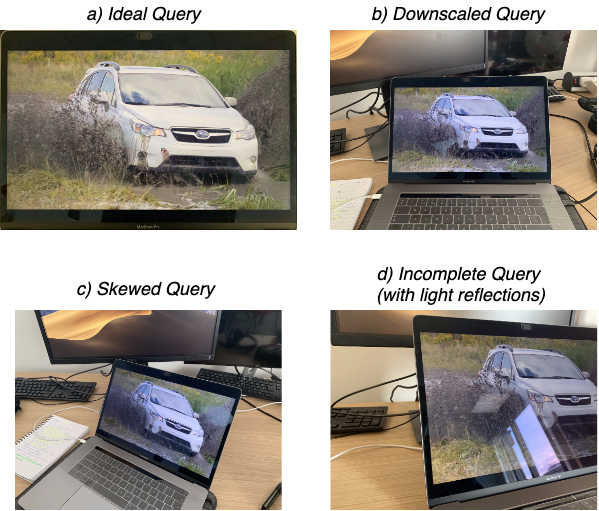
\includegraphics[width=0.8\textwidth]{figures/design/difference-query-video-issues.png}}
\caption{\label{fig:difference-query-video-issues}Different types of video queries, emphasising the contrast between what an idea query and poor quality queries would look like.}
\end{figure}

On the grounds that the system should expect the worst case query, down-scaled and skewed queries should always be considered as the norm. Ideal queries are rare as they depend on competent users. However, incomplete queries as shown in Figure \ref{fig:difference-query-video-issues}d should not be accounted for as it is near-impossible to match such a query to a database video accurately. Therefore, based on this analysis, the assumption that automatically selecting the ROI is a very complex task on its own can be made. Indeed, automatically detecting the edges of different screens to select the video being played as the ROI could grow to be even more intricate than the CBVR system itself. As a result, the ROI should be manually selected by choosing points on the query video to draw a contour around the screen. 

\subsection{Interface}

With Python being the chosen programming language to implement the system and the type of query videos being decided, the next decision is the type of interface that is used to present the results. Although it was specified in Chapter \ref{ch:chapter1} that the system is meant to target mobile devices, creating a mobile application is a waste of time and resources for a project with such a narrow time frame. Although Python offers many choices of creating native GUIs using frameworks such as Tkinter, PyQt or WxPython, or merely creating HTML websites, building a graphical interface would take as much time as developing the entire system pipeline. Indeed, the primary goal is to complete the different phases of the pipeline that process and match a query video to a database video. Spending time on designing a GUI\footnote{Graphical User Interface} for a mobile device is unnecessary as the objective is not to create a commercial application that can be tested with users, as established in the requirements NF2, but to develop the matching algorithm that would work in the background of such an application.\\

The only pieces of information that need to be displayed are the following:
\begin{itemize}
    \item Progress of current phase, e.g. during the offline feature extraction phase, specify how many videos have been processed and how many are left (see requirement F5). Visual cues, such as spinners, to can be used to indicate that work is being carried out by the program.
    \item Histograms: display the generated histograms for each video.
    \item Manual Cropping: display the video to have the user manually select the region of interest.
    \item Results (see requirement F9):
    \begin{itemize}
        \item The distance measurements between the query video and each database videos, while specifying which distance metric is used. Elegant output techniques such as tables could be used to display the results to satisfy requirement NF3.
        \item The final result, which should correspond to a thumbnail of the matched video.
        \item Additional data to measure the efficiency, e.g. the runtime and the accuracy (comparison of the number of true positives and the number of false positives)
    \end{itemize}
\end{itemize}

Most of the information previously mentioned can be displayed directly in the console, such as the current phase progress, the distance measurements and the efficiency results. The only graphical requirements are for the manual query cropping, the histograms and the final result output. The OpenCV GUI functions can be used to display the video in a new window and to manually draw the contour of the region of interest as automatically detecting the edges of the screen in the query video would be a very complicated task on its own. Regarding the histograms and the final result, it is crucial to show visual representations of the histograms and the matched video as it was noticed that during the demonstration of progress in February, only printing the title of the matched video did not provide a sense of accomplishment. Therefore, displaying the histograms and the matched video result can be done through MatplotLib, which is a library used to display plots (histograms) and images (thumbnail of the matched video). The combination of a CLI-based application supported by a few graphical interfaces meet requirement F16, while requirement F19 will only be fulfilled if time allows it as it is a low-priority requirement.

\subsection{Feature Storing File Type}
\label{sec:design-feature-storing-file-type}

The features extracted during the offline feature extraction phase (see Section \ref{sec:design-offline-feature-extraction}) and used during the online retrieval phase (see Section \ref{sec:design-online-retrieval}) can either be stored in text files or binary files. Due to the small amount of spread data (three histograms for each video) and the advantages of being able to view the data being written to the text files for debugging purposes, plain text files are the chosen file types for storing the features extracted from the database videos, satisfying requirement F3. Additionally, now that Python has been chosen as the programming language, functions from the Numpy library can be used to quick I/O operations when saving the data in plain text files, fulfilling requirement F4. For a complete review of the pros and cons between text files and binary files, see Appendix \ref{ch:appendix-comparison-text-vs-binary}.\\

\subsection{Database videos}

Although the goal of the project is to work with feature-length movies, the system will mainly be tested with short videos ranging between 7 and 14 seconds (see requirement F25). Indeed, using feature-length movies is not necessary to test the different stages of the system pipeline, and would not meet requirement F24 since they are copyrighted and not re-usable. Therefore, free stock footage from \textit{Pexels Video}\footnote{Pexels Video: \url{https://www.pexels.com/videos/}} is used instead to populate the database. Feature-length movies can be used to test the database pre-processing phase rather than the entire pipeline (see requirement F27), while the short videos can be used to test the offline feature extraction and online retrieval phases.

\section{Chosen Solution}

\begin{enumerate}
    \item \underline{\textbf{Offline Feature Extraction Phase}}:
    \begin{enumerate}
        \item \textbf{Types of feature}: static colour features in form of colour histograms
        \item \textbf{Types of Histograms}:
        \begin{enumerate}
            \item Grey scale
            \item RGB
            \item HSV
        \end{enumerate}
        \item \textbf{Compact Signature}: Averaged histogram
    \end{enumerate}
    \item \underline{\textbf{Online Retrieval}}: Distance metrics between histograms.
    \item \underline{\textbf{Query Video Pre-Processing}}: 
    \begin{itemize}
        \item Video stabilisation,
        \item ROI selection: manual.
    \end{itemize}
    \item \underline{\textbf{Programming Language}}: Python 3.7\footnote{Version 3.7 is the latest stable release of Python, satisfying NF1.}
    \item \underline{\textbf{Interface}}: Mainly command line for printing data, along with OpenCV GUI for the query video cropping and MatplotLib for displaying the histograms and results.
    \item \underline{\textbf{Feature Storing File Type}}: Plain Text (``.txt'') files.
    \item \underline{\textbf{Database Videos}}: 50 license-free short videos.
\end{enumerate}

\section{Summary}

With the main design aspects of the system pipeline phases laid out, along with an outline of the various system components such as the query video pre-processing operations, programming language, type of interface, type of storage feature file and type of videos used to populate the database, the system can finally be implemented in the next chapter.
